\documentclass[11pt,letterpaper,titlepage]{article}
\usepackage{fancyhdr}
\usepackage[left=0.75in, right=0.75in, bottom=1.0in]{geometry}
\usepackage{lastpage}
\usepackage{titleref}
\usepackage{booktabs}
\usepackage{appendix}

\appendixtitleon
\appendixtitletocon

\makeatletter

%================== List of figures and tables mods
\usepackage{tocloft}
\usepackage[labelfont=bf]{caption}

\renewcommand{\cftfigpresnum}{Figure\ }
\renewcommand{\cfttabpresnum}{Table\ }

\newlength{\mylenf}
\settowidth{\mylenf}{\cftfigpresnum}
\setlength{\cftfignumwidth}{\dimexpr\mylenf+1.5em}
\setlength{\cfttabnumwidth}{\dimexpr\mylenf+1.5em}



%=================== Graphics
\usepackage{graphicx}
\usepackage[breakwords]{truncate}
\usepackage{float}
\usepackage{array}
\usepackage{amsmath}
\usepackage{mdframed}
\usepackage{fancyvrb}
\usepackage{float}
\usepackage{cancel}
\usepackage{amssymb}
\graphicspath{ {images/} }
\usepackage[usenames,dvipsnames,svgnames,table]{xcolor}
\usepackage[defaultlines=2,all]{nowidow}
\usepackage{listings}
\usepackage{color}
\definecolor{Brown}{cmyk}{0,0.81,1,0.60}
\definecolor{OliveGreen}{cmyk}{0.64,0,0.95,0.40}
\definecolor{CadetBlue}{cmyk}{0.62,0.57,0.23,0}
\usepackage{pdflscape}
\usepackage{relsize}
\usepackage{verbatim}
\usepackage{tabto}
\usepackage{upgreek}
\usepackage{enumitem}

%=================== Settings
\renewcommand{\baselinestretch}{1.2}
\definecolor{gray}{rgb}{0.4 0.4 0.4}
\newcommand{\stimes}{{\times}}

\begin{document}
\newcommand{\NSCDOCNUMBR}{NSC-REP-15-X}         %Put document number here
\newcommand{\NSCDOCSUBJT}{TECHNICAL REPORT: }   %Put document subject here
\newcommand{\NSCDOCTITLE}{The Surface Remeshing Module in $ChiTech$}       %Put document title here
\newcommand{\NSCDOCDATE} {August, 2018}    %Put document date here
\newcommand{\NSCDOCREV}  {Rev 1.02} %Put revision number here

\lstset{language=C++,frame=ltrb,framesep=2pt,basicstyle=\linespread{0.8} \small,
	keywordstyle=\ttfamily\color{OliveGreen},
	identifierstyle=\ttfamily\color{CadetBlue}\bfseries,
	commentstyle=\color{Brown},
	stringstyle=\ttfamily,
	showstringspaces=true,
	tabsize=2,}


%################################# TITLE PAGE ########################
\begin{titlepage}
	\pagestyle{fancy}
	\vspace*{1.0cm}
	\centering
	%\includegraphics{NSC_Logo} \par
	\vspace{1cm}
	%\centering
	%{\Large\bfseries  \NSCDOCNUMBR   \par}
	\vspace{.25cm}
	%\centering
	{\Large\bfseries  \NSCDOCSUBJT \par} 
	{\Large\bfseries \NSCDOCTITLE  \par}
	\vspace{1cm}
	{\Large \NSCDOCDATE \par}
	\vspace{1.0cm}
	{\Large Jan Vermaak \par}
	{\Large \NSCDOCREV \par}
		
	\begin{comment}
	\renewcommand{\arraystretch}{2.0}
	\begin{tabular}{| m{2.5cm} | m{4.5cm} | m{4.5cm} |}
		\cline{2-3}
		\multicolumn{1}{c|}{} & \bfseries{Name} & \bfseries{Signature \& Date} \\ \hline
		\bfseries{Prepared} &     &     \\ \hline
		\bfseries{Reviewed} &     &     \\ \hline
		\bfseries{Reviewed} &     &     \\ \hline
	    \bfseries{Approved} &     &     \\ \hline
	\end{tabular} \par
	
	\begin{center}
		\begin{minipage}[c]{0.55\textwidth}
	
			\begin{figure}[H]
			
				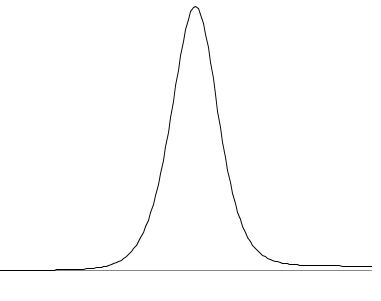
\includegraphics{Logo.png}
			\end{figure}
		\end{minipage}
	\end{center}
	\vspace{2cm}
	\end{comment}
	%NSC-FRM-15-1 Rev.1
\end{titlepage}


\pagestyle{fancy}
\rfoot{Page \thepage \ of \pageref{LastPage}}
%\cfoot{NSC-FRM-15-1 Rev.1}
\cfoot{}
\lfoot{\truncate{14cm}{\NSCDOCTITLE}}
\rhead{}
\chead{\currentname}
\lhead{}
\renewcommand{\footrulewidth}{0.4pt}
\tableofcontents
\addtocontents{toc}{~\hfill\textbf{Page}\par}

\listoffigures
\listoftables
\chead{Contents}


\newpage
\chead{1 Fundamental Mission}
\section{Fundamental Mission}



Let us begin with the fundamental mission of the Surface Remesher Module (SRM). This Module should be able to take a surface mesh, which is normally generated by a CAD or animation package, and retriangulate all the faces so that it is more convenient for volume meshing. This mission is best described graphically as shown in Figure \ref{figure:Mission}. In the sections that follow different methods of surface remeshing will be explored.

\begin{center}
	\begin{minipage}[c]{0.82\textwidth}

		\begin{figure}[H]
		
			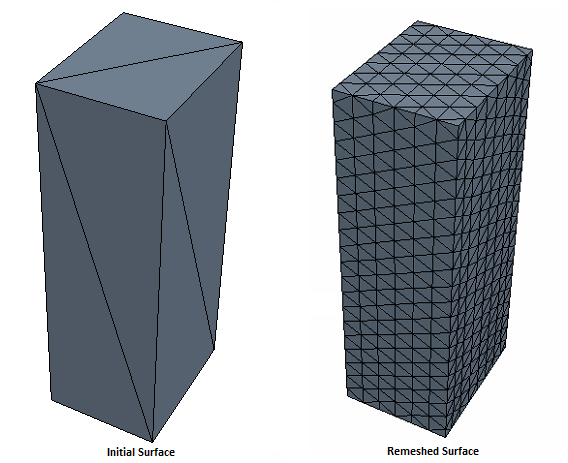
\includegraphics{Mission.png}
			\caption{Example of a surface remeshing operation.}
			\label{figure:Mission}
		\end{figure}
	\end{minipage}
\end{center}

\newpage
\subsection{Format of the input geometry}
For this whitepaper we will only consider geometry supplied by ASCII based formats, more specifically the Wavefront (\textit{.obj}) format, which is easily exported by the 3D modeling tool blender \cite{blender}. The format lists all the vertices of the geometry followed by, a list of normal vectors and (optionally) a list of UV vertices for texture mapping. Lastly the format provides a list of faces. Each face contains three groups of information: vertex, UV-vertex and vertex-normal (i.e. 5/2/1 or 5//1 if there are no UV-vertices). A sample of the format is shown below:

\begin{verbatim}
# Blender v2.79 (sub 0) OBJ File: ''
# www.blender.org
o Plane_Plane.003
v -4.000000 -4.000000 1.000000
v 4.000000 -4.000000 1.000000
v -4.000000 4.000000 1.000000
v 4.000000 4.000000 1.000000
v -3.000000 -3.000000 1.000000
v 3.000000 -3.000000 1.000000
v -3.000000 3.000000 1.000000
v 3.000000 3.000000 1.000000
vn 0.0000 0.0000 1.0000
s off
f 5//1 3//1 1//1
f 4//1 7//1 8//1
f 1//1 2//1 6//1
f 5//1 7//1 3//1
f 1//1 6//1 5//1
f 6//1 2//1 4//1
f 4//1 3//1 7//1
f 8//1 6//1 4//1
\end{verbatim}

\noindent The information contained in this format is enough to display the surface in a 3D rendering program.

\newpage
\subsection{ChiTech's internal storage format}
Fundamentally a surface mesh is stored in the \textit{CHI\_SURFACE} class,

\begin{lstlisting}{language=C++}
class CHI_SURFACE
{
 public:
	.
	.	
	//===================================================== Raw data
	CHI_VECTOR<GLfloat>		vertexStack;			
	CHI_VECTOR<GLfloat>		tVertexStack[10];		///< Stacks for texture channel vertices.
	CHI_VECTOR<GLfloat>     normalStack;           
	CHI_VECTOR<CST_FACE>	faceStack;			
	.
	.
};
\end{lstlisting}

\noindent And triangles are stored in the \textit{CST\_FACE} structure,

\begin{lstlisting}{language=C++}
struct CST_FACE
{
	int						vertex[3];
	.
	.
	int                     normal[3];
	.
	.
	float                   faceNormal[3];
	int                     edges[3][3];
	.
	.
};
\end{lstlisting}

\newpage
\chead{2 Finding co-planar collections of faces}
\section{Finding co-planar collections of faces}

\begin{lstlisting}{language=C++}
CHI_VECTOR<CHI_FACELIST> coPlanarFaceCollections;
CollectCoPlanarFaces(&coPlanarFaceCollections);
\end{lstlisting}
For each face $F_f$ we can explore all its attached faces by identifying shared vertices. We can create collections of co-planar faces by using their respective normals, $N_f$, and hence arrive at planes that have contours in need of discretization. Some collections can be as few as a single face. In order to find the normal (since we cannot use the graphical normal) we first find the vector, $v_{01}$, from vertex 0 to vertex 1 then the vector, $v_{12}$, from vertex 1 to vertex 2:
$$
\bar{v}_{01}=\bar{v}_{1}-\bar{v}_{0}=[v_{1x},v_{1y},v_{1z}] - [v_{0x},v_{0y},v_{0z}]
$$
$$
\bar{v}_{12}=\bar{v}_{2}-\bar{v}_{1}=[v_{2x},v_{2y},v_{2z}] - [v_{1x},v_{1y},v_{1z}]
$$
We can then find the normal from the cross-product of these vectors:
$$
\hat{n}_{face}=\frac{\bar{v}_{01} \times \bar{v}_{12}}
                    {||\bar{v}_{01} \times \bar{v}_{12}||}
$$
Two faces, faces $F_a$ and $F_b$, lie in the same plane if:
$$
\biggr | \hat{n}_a  \bullet \hat{n}_b \biggr | < 1-\epsilon
$$
Of course we have to deal with precision issues and therefore these normals have to be compared component wise with some tolerance $\epsilon=${$\pm 0.000001 \ cm$}. With this approach we can end up with a plane collection as shown in Figure \ref{figure:FindCoPlanar} below.

\begin{center}
	\begin{minipage}[c]{0.4\textwidth}

		\begin{figure}[H]
		
			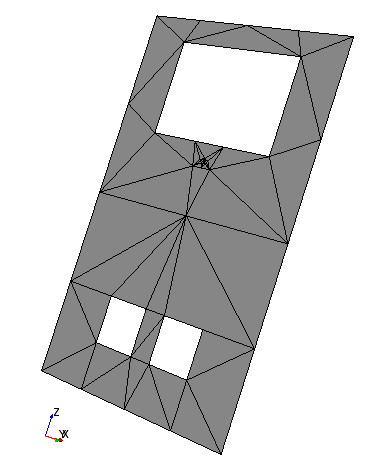
\includegraphics[width=2.2in]{FindCoPlanar.png}
			\caption{Example of a collection of coplanar faces.}
			\label{figure:FindCoPlanar}
		\end{figure}
	\end{minipage}
\end{center}
\newpage
\chead{3 Splitting by Patch}
\noindent
There is however a complication with this approach. What will happen when some faces have normals pointing in the same direction but they are at either a different depth or not connected to the same contiguous collection of faces (see figure \ref{fig:findcoplanar2})? They will of course still be present in the co-planar collection. To solve this problem we need to split non-contiguous collections into \textbf{Patches}.

\begin{figure}[H]
    \centering
    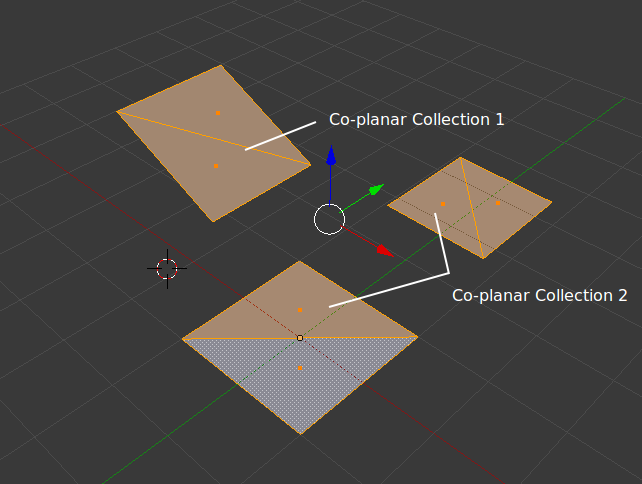
\includegraphics[width=0.7\linewidth]{FindCoPlanar2}
    \caption{Co-planar collections with disjointed areas.}
    \label{fig:findcoplanar2}
\end{figure}


\vspace{1cm}
\section{Splitting by Patch}
\begin{lstlisting}{language=C++}
CHI_VECTOR<CHI_PATCH> patchCollections;
CreatePatchList(&coPlanarFaceCollections,&patchCollections);
\end{lstlisting}

\vspace{0.5cm}
\begin{lstlisting}{language=C++}
struct CHI_PATCH
{
	Eigen::Vector3f normal;
	CHI_VECTOR<CST_FACE> faceList;
	CHI_VECTOR<int> edges;
	CHI_VECTOR<CHI_COLINEDGELIST> colinearEdges;
	CHI_VECTOR<CHI_EDGELOOP> edgeLoops;
	CHI_VECTOR<int> essentialVertices;
	CHI_VECTOR<int> lexicalListOfVertices;
};
\end{lstlisting}

\noindent
The easiest way to split by patch, assuming no duplicate vertices exist is to assemble the patches from the given collection of co-planar faces. If a given patch finds no more connections and there are still unused faces in the co-planar collection (not assigned to patches yet) then a new patch can be created. The pseudo-code for this is shown below.
\newline

\begin{lstlisting}
for (i=0;i<coplanarcollections.itemCount;i++)
{
	DynamicArray patchList;
	currentCoplanarCollection = coplanarcollections.GetItem(i);
	
	if (patchList.itemCount==0)
	{
		patch1 = patchList.NewItem
		firstFace = currentCoplanarCollection.GetItem(0);
		patch1.AddFace(firstFace);
		
		unusedFaces = currentCoplanarCollection.Items(1 to totalItems);
		
		while (unusedFaces.itemCount>0)
		{
			updateMade=false;
			for each patch
			{
				for each face in patch
				{
					for each unusedFace
					{
						if (unusedFace connected to patch->face)
						{
							add unusedFace to patch;
							updateMade = true;
						}
					}
				}
			}
			if (not updateMade && unusedFaces.itemCount>0)
			{
				newPatch = patchList.NewItem;
				newPatch.AddFace(unusedFaces.PopItem);
			}
		}
	}
}
\end{lstlisting}



\newpage
\section{Obtaining Edge-loops and Essential vertices}
\begin{lstlisting}{language=C++}
FindOpenEdges(&patchCollections);
FindCoLinearEdges(&patchCollections);
FindEdgeLoops(&patchCollections);
ListEssentialVertices(&patchCollections);
\end{lstlisting}
For each patch $p$ we have a point-set $\mathcal{P}^{init}$ that is used to define the initial triangulation $\uptau^{init}$. Each triangulation $\uptau$, which can be an \textit{affine hull} or a \textit{convex hull}, is a combination of numerous $\tau$-simplexes (triangles $\tau(p_a,p_b,p_c)$) and $\sigma$-simplexes (edges $\sigma(p_a,p_b)$). Open-edges $\sigma^{open}$, edges that are part of only one triangle, can be collected and connected to form edge-loops

\begin{equation*}
\begin{aligned}
\sigma_j^{loop} 
&=\sigma_0^{open}  &&,p_b^{N-1}=p_a^0, \ p_b^0=p_a^1 \\
&+\sum_{i=1}^{N-2} \sigma_i^{open} &&,p_b^{i-1} = p_a^{i}, \ p_b^i = p_a^{i+1} \\
&+\sigma_{N-1}^{open}  &&,p_b^{N-2}=p_a^{N-1}, \ p_b^{N-1}=p_a^0 \\
\end{aligned}
\end{equation*}
\newline
\noindent Edge-loops are used to define simplexes that need to be respected during triangulation and will be used to recover the initial affine hull. The essential vertices of the original affine (see figure \ref{fig:EdgeLoops}) hull is also the essential vertices of the edge-loops and to obtain the essential vertices of the edge-loops one needs to combine co-linear edges and obtain the vertices that maximizes the length of this edge.

\begin{figure}[h]
    \centering
    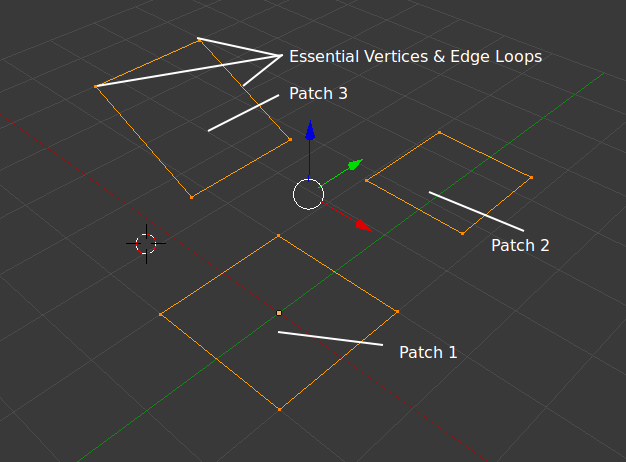
\includegraphics[width=0.7\linewidth]{EdgeLoops.png}
    \caption{Collection of edge-loops and essential vertices for each patch.}
    \label{fig:EdgeLoops}
\end{figure}


\newpage 
\chead{5 Lexicographical Triangulation}
\section{Lexicographical Triangulation}

\noindent For each patch $p$ of the initial triangulation we copy the patch's essential vertices and edge-loops to the remeshed surface $\uptau^{new}$ along with a re-indexing of the vertices.

\vspace{0.5cm}
\begin{lstlisting}{language=C++}
this->remeshedSurface = new CHI_REMESHEDSURFACE;
CopyInformationToRemeshedSurface(&patchCollections, remeshedSurface);
\end{lstlisting}


\begin{figure}[h]
\centering
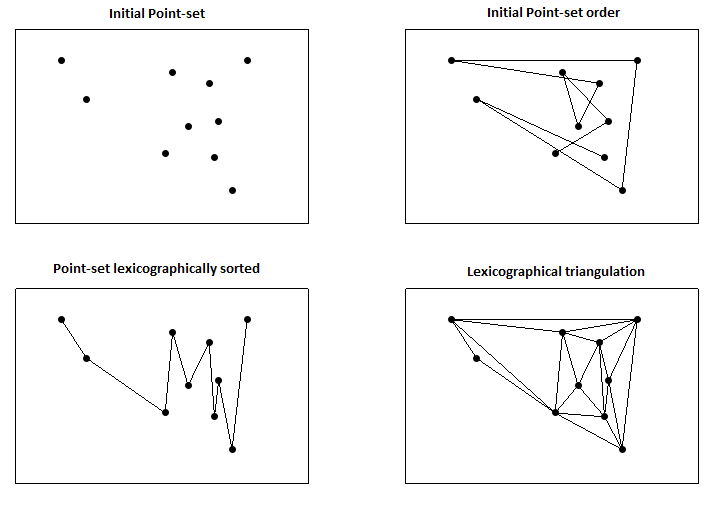
\includegraphics[width=0.8\linewidth]{LexicoGraphical}
\caption{Lexicographical triangulation of a random point-set.}
\label{fig:LexicoGraphical}
\end{figure}

\subsection{Project 3D vertices to 2D}

\vspace{0.5cm}
\begin{lstlisting}{language=C++}
CHI_VECTOR<float> Pstar;
CHI_PATCH* curPatch = mesh->patches.GetItem(p);
Project3DVerticesTo2D(mesh,&Pstar,curPatch);
\end{lstlisting}


\noindent The 2D triangulation algorithm does not work with 3D points and therefore it is needed to project the 3D vertices of each patch to a 2D space. We start by defining the up-vector as:

\begin{equation*}
\hat{k} = \hat{n}_{patch}
\end{equation*}

\noindent Where $\hat{n}_{patch}$ is the normal of the patch being remeshed (each face in this patch has the same normal).

Calculating $\hat{i}$ reduces to a selection of 3 choices:
\begin{itemize}
\item Leave $\hat{i}$ un-altered in the 2D plane (i.e. $\hat{i}=[ 1, 0, 0]$).
\item Choose the most dominant edge in one of the edge-loops (i.e. longest length and x-axis dominant)
\item Use a predesignated edge
\end{itemize}

\vspace{0.5cm}
\noindent With the $\hat{i}$ selection made we can then calculate 

$$
\hat{j} = \hat{k} \times \hat{i}
$$

\noindent Given the centroid $c_0=\frac{1}{N} \sum_{i=0}^{N-1} p_i$, we can now calculate a projected point-set $\mathcal{P}^*$ as follows:
$$
PC_i = p_i - c_0 
$$
\begin{equation*}
\begin{aligned}
p_i^* = [PC_i \bullet \hat{i} ] \cdot \hat{i} 
+ [PC_i \bullet \hat{j} ] \cdot \hat{j}
+ [0] \cdot \hat{k}
\end{aligned}
\end{equation*}

\vspace{0.5cm}
\noindent Note that the projected point-set $\mathcal{P}^*$ has the same index as the original point set $\mathcal{P}$ and can therefore operate on the same lexicographical sorting.


\subsection{Sort points lexicographically}

\vspace{0.5cm}
\begin{lstlisting}{language=C++}
CHI_VECTOR<int> lexList;
SortLexicographically2D(&Pstar,curPatch,&lexList);
\end{lstlisting}


\noindent Sort the projected point-set $P^*$ first by $x$ then by $y$.

\subsection{Orient2D for checking clock-wise triangles}
Suppose we have vertices $v_a$, $v_b$ and $v_c$ in $\mathcal{P}^*$. If we want to investigate the orientation of a triangle formed using $a$, $b$ and $c$ we can form two vectors 

$$ba=b-a$$
$$cb=c-b$$

\noindent With the orientation given by:

$$Orient2D(a,b,c) = \hat{k} \bullet (ba \times cb) $$

\noindent Or equivalently (and more efficiently):

\begin{equation*}
Orient2D(a,b,c)=
\begin{vmatrix}
a_x &a_y &1\\
b_x &b_y &1\\
c_x &c_y &1\\
\end{vmatrix}
\end{equation*}

\subsection{Create initial Triangle}

\begin{lstlisting}{language=C++}
CreateInitialTriangle(&Pstar,curPatch,&lexList);
\end{lstlisting}

\noindent
Initially, all the vertices in $\mathcal{P}^*$ are unused and therefore we can use the first very first lexicographically sorted vertex as the starting point $v_a$ of the first triangle.

In order to ensure a right-hand-rule (RHL) compliant triangle we need to make a first-line check that prevents the second vertex $v_b$ from having the same $x$ as $v_a$ because this will lead to a co-linear point selection $abc$. 

The third vertex $v_c$ has no limitation other than it cannot be the same as $v_b$. The final triangle though needs to comply with the RHL and therefore we need to check 

$$ AB = v_b - v_a $$
$$ BC = v_c - v_b $$
$$ require \ (AB \times BC)\bullet \hat{k} > 0$$

The prototype-code for this is:
\begin{lstlisting}{language=C++}
hullPoint1 =  lexlist(1);
hullPoint2 = -1;
hullPoint3 = -1;
for i=2:N
    if (points(lexlist(1),1)~=points(lexlist(i),1)) then
        hullPoint2=lexlist(i);
        break;
    end
end
for i=2:N
    a=points(lexlist(i),:);
    b=points(hullPoint1,:);
    c=points(hullPoint2,:);
    orientation = Orient2D(a,b,c);
    
    if (   (lexlist(i)~=hullPoint2)   )
        hullPoint3=lexlist(i);
        if (orientation>0) then
            tempHullpoint=hullPoint2;
            hullPoint2 = hullPoint3;
            hullPoint3 = tempHullpoint;
            disp("Vertices flipped")
        end
        
        break;
    end
end
\end{lstlisting}

\subsection{Create List of unused vertices}

\begin{lstlisting}{language=C++}
GetUnusedVertices(curPatch,&lexList,&unusedVertices);
\end{lstlisting}

\noindent Any vertex that is not connected to a triangle is eligible to be added to the hull of lexicographically triangulated faces. This function can potentially be called multiple times.

\subsection{Iterate until all vertices are used}

\begin{lstlisting}{language=C++}
bool forcestop=false;
while ((unusedVertices.itemCount>0) && (!forcestop))
{
	AttachUnusedVertex(&Pstar,curPatch,&lexList,&unusedVertices);
	ConvexifyHull(&Pstar,curPatch,&lexList);
	GetUnusedVertices(curPatch,&lexList,&unusedVertices);
}
ConvexifyHull(&Pstar,curPatch,&lexList);
\end{lstlisting}

\newpage
\subsubsection{Attach an unused vertex}

\begin{lstlisting}{language=C++}
AttachUnusedVertex(&Pstar,curPatch,&lexList,&unusedVertices);
\end{lstlisting}
Given the next unused vertex $v_i$, we can iterate over the convex-hull's edges to find a convex addition point for $v_i$.

\begin{lstlisting}{language=C++}
hullEdges=FindOpenEdges(out_convexHull);
i=1;
for t=1:(size(hullEdges)(1))
    a=points(out_unusedLexlist(i),:);
    b=points(hullEdges(t,1),:);
    c=points(hullEdges(t,2),:);
    
    orientation = Orient2D(a,b,c);
    
    if (orientation>0) then
        //Tell the owner of the edge that it now has a neighbor
        ownerTriangle = hullEdges(t,3);
        ownerEdgeNo   = hullEdges(t,4);
        out_convexHull(ownerTriangle,3+ownerEdgeNo)=size(out_convexHull)(1)+1;
        
        //Tell the new triangle which neighbor its attaching to
        newTriangle = [hullEdges(t,1) 
        out_unusedLexlist(i) hullEdges(t,2) -1 -1 ownerTriangle]
        
        out_convexHull= [out_convexHull; newTriangle]; //Add triangle
        //Update unused vertices and openEdges
        [out_unusedLexlist]=GetUnusedVertices(in_lexlist,out_convexHull)
        
        hullEdges=FindOpenEdges(out_convexHull);
     
        break;
    end                       
    if ( (size(out_unusedLexlist)(1)==0) )
        break;
    end
end
\end{lstlisting}

\begin{figure}[h]
\centering
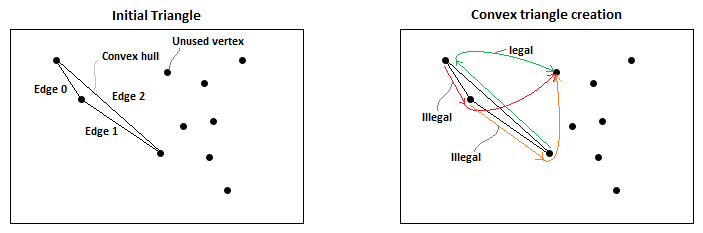
\includegraphics[width=0.8\linewidth]{AttachUnused.png}
\caption{Attaching a triangle.}
\label{fig:AttachUnused}
\end{figure}

\newpage
\subsubsection{Convexifying the hull}

\begin{lstlisting}{language=C++}
ConvexifyHull(&Pstar,curPatch,&lexList);
\end{lstlisting}
The initial triangle will obviously form a convex-hull, however, after subsequent triangle additions the hull might not be convex anymore. When the hull is not convex then the triangle addition can potentially cross existing triangle and therefore an algorithm is required to convexify the hull.

\begin{lstlisting}{language=C++}
hullEdges=FindOpenEdges(out_convexHull);
concaveEdgesFound=%T;
while (concaveEdgesFound)
    concaveEdgesFound=%F;
    for t=1:(size(hullEdges)(1))
        edgeCombo = [hullEdges(t,:)];
        if (t<(size(hullEdges)(1))) then
            edgeCombo = [edgeCombo; hullEdges(t+1,:)];
        else
            edgeCombo = [edgeCombo; hullEdges(1,:)];
        end
        a=in_points(edgeCombo(2,2),:);  b=in_points(edgeCombo(1,1),:);
        c=in_points(edgeCombo(1,2),:);  orientation = Orient2D(a,b,c);
        
        if (orientation>0) then
            concaveEdgesFound=%T;
            //Tell the owner of the edge that it now has a neighbor
            ownerTriangle1 = edgeCombo(1,3); ownerEdgeNo1   = edgeCombo(1,4);
            ownerTriangle2 = edgeCombo(2,3); ownerEdgeNo2   = edgeCombo(2,4);
            out_convexHull(ownerTriangle1,3+ownerEdgeNo1)=size(out_convexHull)(1)+1;
            out_convexHull(ownerTriangle2,3+ownerEdgeNo2)=size(out_convexHull)(1)+1;
            
            //Tell the new triangle which neighbor its attaching to
            newTriangle = [edgeCombo(1,1) 
            edgeCombo(2,2) edgeCombo(1,2) -1 ownerTriangle2 ownerTriangle1]
            out_convexHull= [out_convexHull; newTriangle]; //Add triangle

            //OpenEdges
            hullEdges=FindOpenEdges(out_convexHull);
            break;
        end                  
    end
end
\end{lstlisting}
\begin{figure}[h]
\centering
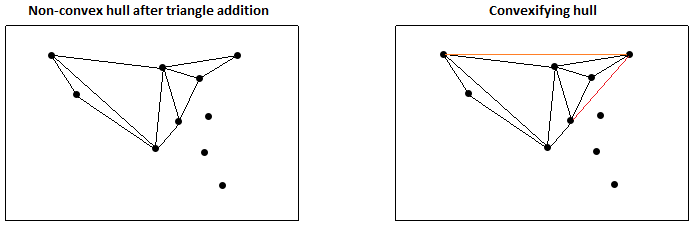
\includegraphics[width=0.8\linewidth]{Convexify.png}
\caption{Convexifying a non-convex hull.}
\label{fig:Convexify}
\end{figure}

\newpage
\chead{6 Make the triangulation Delaunay}
\section{Make the triangulation Delaunay}

Following Lemma 2.3 in \cite{delaunay}, if $\uptau$ is a triangulation of the point-set $S$ then the following are equivalent:

\begin{enumerate}[label=(\roman*)]
\item Every triangle in $\uptau$ is Delaunay
\item Every edge in $\uptau$ is Delaunay
\item Every edge in $\tau$ is locally Delaunay
\end{enumerate}
\noindent Additionally, the simple requirement for an edge to be locally Delaunay can be assured by using the \textit{Edge-flip} algorithm.

An edge of two triangles is locally Delaunay if the smallest circumdisc (of the two triangles) does not contain any vertices of its adjacent triangles (other than those belonging to the edge). An edge of one triangle is always Delaunay.

\subsection{InCircle for finding a non-locally-Delaunay Edge}
Given two triangles $\tau_{abc}$ and $\tau_{cda}$ joined at edge $ac$. The edge is non-locally Delaunay if 

\begin{equation*}
\begin{vmatrix}
a_x &a_y &a_x^2+a_y^2 &1 \\
b_x &b_y &b_x^2+b_y^2 &1 \\
c_x &c_y &c_x^2+c_y^2 &1 \\
d_x &d_y &d_x^2+d_y^2 &1 \\
\end{vmatrix}>0
\end{equation*}

\subsection{Finding non-locally-Delaunay Edges} 
\begin{lstlisting}{language=C++}
CHI_VECTOR<CHI_INTERIOREDGE> non_local_del_edges;
ListNonLocallyDelaunayEdges(&Pstar,curPatch,&non_local_del_edges);
\end{lstlisting}

\noindent This algorithm needs to loop through all interior edges and check for the local-Delaunay condition. If it finds an edge it needs to add the $INTERIOREDGE$ data structure to the list of non-locally-Delaunay edges on the conditions its not already there.

This data structure stores information of the edge's vertices from $v_i$ to $v_f$ as well as the triangle to which the edge belonged when the edge was first found $\tau_1$ and its corresponding neighbor $\tau_2$.
\newline

\begin{lstlisting}{language=C++}
struct CHI_INTERIOREDGE
{
	int vi;
	int vf;
	int tau_1;
	int tau_1_edgeNumber;
	int tau_2;
	int tau_2_edgeNumber;
};
\end{lstlisting}

\noindent The pseudo-code for this algorithm is given below.

\begin{lstlisting}{language=C++}
for each face
	tau_1 = face
	for each edge of the face
		tau_2 = edge-neighbour
		
		a = tau_1->vertex[0];
		b = tau_1->vertex[1];
		c = tau_1->vertex[2];
		d = tau_2->vertex[not a,b or c];
		
		localDelaunay = InCircle(a,b,c,d);
		
		if (localDelaunay>0.000001)
			Check for duplicate edge
			Add to list of non-loc-del-edges
		end
	end
end
\end{lstlisting}

\subsection{Edge-Flip}

\begin{lstlisting}{language=C++}
EdgeFlip(curPatch,&non_local_del_edges);
\end{lstlisting}

\begin{figure}[h]
\centering
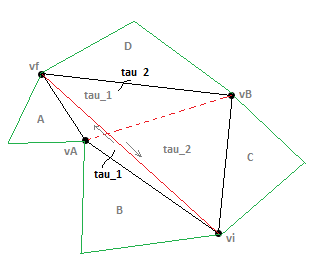
\includegraphics[width=0.5\linewidth]{EdgeFlipRef}
\caption{Reference schematic for the edge-flip algorithm.}
\label{fig:EdgeFlipRef}
\end{figure}

\noindent Given a non-locally-Delaunay edge defined from $v_i$ to $v_f$, $\tau_1$ and $\tau_2$ is defined by two additional vertices $v_A$ and $v_B$. Because of the pure clock-wise assignment of triangles the orientation as in figure \ref{fig:EdgeFlipRef} will always be valid. According to this orientation $\tau_1$ needs to be transformed from $v_i,v_f,v_A$ to $v_A,v_B,v_f$ and similarly $\tau_2$ needs to be transformed from $v_f,v_i,v_B$ to $v_B,v_A,v_i$. Neighbors B and D will also need to be informed that their neighbors have been exchanged.

\newpage
\noindent The pseudo-code for this is shown below:
\begin{lstlisting}{language=C++}
get tau_1 and tau_2
find neighbors A,B,C,D
find v_A and v_B
Reassign tau_1 and its edge information
Reassign tau_2 and its edge information
Update neighbors B and D
\end{lstlisting}


\newpage
\chead{7 Mesh refinement}
\section{Mesh refinement}

\subsection{Mesh quality metrics}
The optimum triangular element is one that is close to a equilateral triangle.

\begin{figure}[h]
\centering
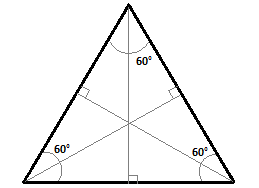
\includegraphics[width=0.4\linewidth]{Equilateral.png}
\caption{An equilateral triangle.}
\label{fig:Equilateral}
\end{figure}

\noindent
For such a triangle, with side length $\ell$ the circumcircle has all of the vertices on its circumference and the radius $R_c$ is

$$\frac{\ell/2}{R_c} = cos(30^\circ)=\frac{\sqrt{3}}{2}$$
$$\therefore R_c = \frac{1}{\sqrt{3}}\ell$$
\newline
This corresponds to a radius-to-edge ratio, $\rho$, of $0.5773$ and a ratio from which one departs rapidly when one of the triangle's sides grow. Therefore the radius-to-edge ratio $\rho$ is a good measure of a triangle's aspect ratio.



\newpage
\chead{References}
\begin{thebibliography}{1}

	\bibitem{blender} {\em Blender - a 3D modelling and rendering package}, Blender Online Community, Blender Foundation, Blender Institute, Amsterdam, 2018
	
	\bibitem{delaunay} Cheng et al, {\em Delaunay Mesh Generation}, Chapman \& Hall/CRC Computer \& Information Science Series, 2013
	
	
\end{thebibliography}





\end{document}